% !TEX root = ./main.tex                             %WICHTIG FÜR VSCODE!!!!!!!!!!!!
\documentclass[runningheads]{llncs}


%
\usepackage[T1]{fontenc}
\usepackage{graphicx}
\usepackage{comment}
\usepackage{hyperref}
\usepackage{color}
%\renewcommand\UrlFont{\color{blue}\rmfamily}


\begin{document}


\title{Fahrgastüberwachung im ÖPNV}
\author{Tim Pröpper}
\institute{ Ostfalia Hochschule Wolfenbüttel, Am Exer 2, Wolfenbüttel, Braunschweig
    \email{info@ostfalia.de}\\
    \url{https://www.ostfalia.de}}

{\def\addcontentsline#1#2#3{}\maketitle}            % typeset the header of the contribution


\begin{abstract}
    The abstract should briefly summarize the contents of the paper in
    150--250 words.

    \keywords{ÖPNV  \and Überwachung \and Datenschutz.}
\end{abstract}

\setcounter{tocdepth}{2}
\tableofcontents
\setcounter{page}{0}
\section{Einleitung}
Der Anteil der Überwachung im öffentlichen Personennahverkehr hat mit fortschreitender Digitalisierung beständig zugenommen.

-- hat er das?
-- Abkürzungen: DSGVO, ÖPNV, BDSG

-- Motivation

-- Ziel der Hausarbeit: Anwendung von Methoden

-- Aufbau: Übersicht, Analyse von 2 Risiken inklusive Maßnahmen


\begin{table}
    \caption{Table captions should be placed above the
        tables.}\label{tab1}
    \begin{tabular}{|l|l|l|}
        \hline
        Heading level     & Example                                          & Font size and style \\
        \hline
        Title (centered)  & {\Large\bfseries Lecture Notes}                  & 14 point, bold      \\
        2nd-level heading & {\bfseries 2.1 Printing Area}                    & 10 point, bold      \\
        3rd-level heading & {\bfseries Run-in Heading in Bold.} Text follows & 10 point, bold      \\
        4th-level heading & {\itshape Lowest Level Heading.} Text follows    & 10 point, italic    \\
        \hline
    \end{tabular}
\end{table}
\section{Übersicht}
\subsection{Einsatzgebiet}
Öffentlicher Personennahverkehr bezeichnet den \glqq{} räumlichen Bereich zur Beförderung von Personen im Berufs-,
Ausbildungs-, Einkaufs- und sonstigen alltäglichen Verkehr mit Fahrzeugen des Straßen-, Schienen- und Schiffsverkehrs (Fähren) im Linienverkehr.
\grqq{} \cite{Dr.FriedrichvonStackelbergDr.RobertMalina.2018}
Die Einsatzgebiete von Fahrgastüberwachung betreffen alle dem entsprechenden Verkehrsbetrieb zugehörigen Gebiete, in welchen sich Personen aufhalten.
Dies umfasst also die Haltestellen sowie die Verkehrsmittel selbst.
\subsection{Rechtliche Rahmenbedingungen}
Die rechtliche Grundlage für die Fahrgastüberwachung ist durch §4 Bundesdatenschutzgesetz Abs. 1 S. 2 \glqq{} Videoüberwachung öffentlich zugänglicher Räume\grqq{}
gegeben. Genauer heißt es dort:\\
\glqq{}Bei der Videoüberwachung von
\begin{enumerate}
    \item öffentlich zugänglichen großflächigen Anlagen, wie insbesondere Sport-,\\ Versammlungs- und Vergnügungsstätten, Einkaufszentren oder Parkplätzen, oder
    \item Fahrzeugen und öffentlich zugänglichen großflächigen Einrichtungen des öffentlichen Schienen-, Schiffs- und Busverkehrs
\end{enumerate}
gilt der Schutz von Leben, Gesundheit oder Freiheit von dort aufhältigen Personen als ein besonders wichtiges Interesse.\grqq{} \cite{Bundestag.2018}\\
Ebenfalls die Fahrgastüberwachung betreffend ist die europäische Datenschutzgrundverordnung bezüglich Artikel 6 \glqq{}Rechtmäßigkeit der Verarbeitung\grqq{},
Artikel 13, 14\glqq{}Informationspflicht\grqq{} und Artikel 17 \glqq{}Recht auf Löschung\grqq{} \cite{EuropaischeUnion.}

\subsection{Architektur}
In Abbildung~\ref{fig:architektur} wird der Systemaufbau dargestellt. Hierbei wird unterschieden zwischen dem lokalen Aufbau, der an den Fahrzeugen und Haltestellen
anzufinden ist. Über ein Netzwerk ist jedes lokale System mit der zentralen Leitstelle verbunden.

Ein lokales System hat in der Regel mehrere Kameras (analog oder digital) verbaut. Das Bild analoger Kameras muss vor Anbindung an das Netzwerk digitalisiert werden.
Optional in den lokalen System sind eine Anzeige für z.B. deb Fahrer des Busses, sowie Mikrofone, welche in den Kameras integriert sein können.

In der zentralen Verwaltung stehen die Server, welche die Videoaufnahmen verwalten sowie das \glqq{}Langzeit-Archiv\grqq{}. In diesem werden die Aufnahmen bis zur Löschung aufbewahrt.
Über den Dauer bis zur Löschung der Daten heißt bisher Uneinigkeit, gemäß § 27 Bundespolizeigesetz (BPolG) ist eine Speicherung von bis zu 30 Tagen zulässig. In  §6b Abs. 5 BDSG
steht dem die unweigerliche Löschung der Daten gegenüber. In der \glqq{}Orientierungshilfe zur Videoüberwachung\grqq{} der Datenschutzbeauftragten von Niedersachsen wird eine maximale
Speicherdauer von 48 Stunden angegeben\cite{DanielaWindelband.20.April2016}. Neben der Darstellung der Videos sind auch technische Möglichkeiten zur Auswertung der Videos geschaffen.
Auswertung umfasst nicht automatisch die automatische Analyse der Daten, sondern beschreibt vielmehr das Betrachten und Beurteilen dieser durch einen Mitarbeiter.

\begin{figure}[ht]
    \begin{center}
        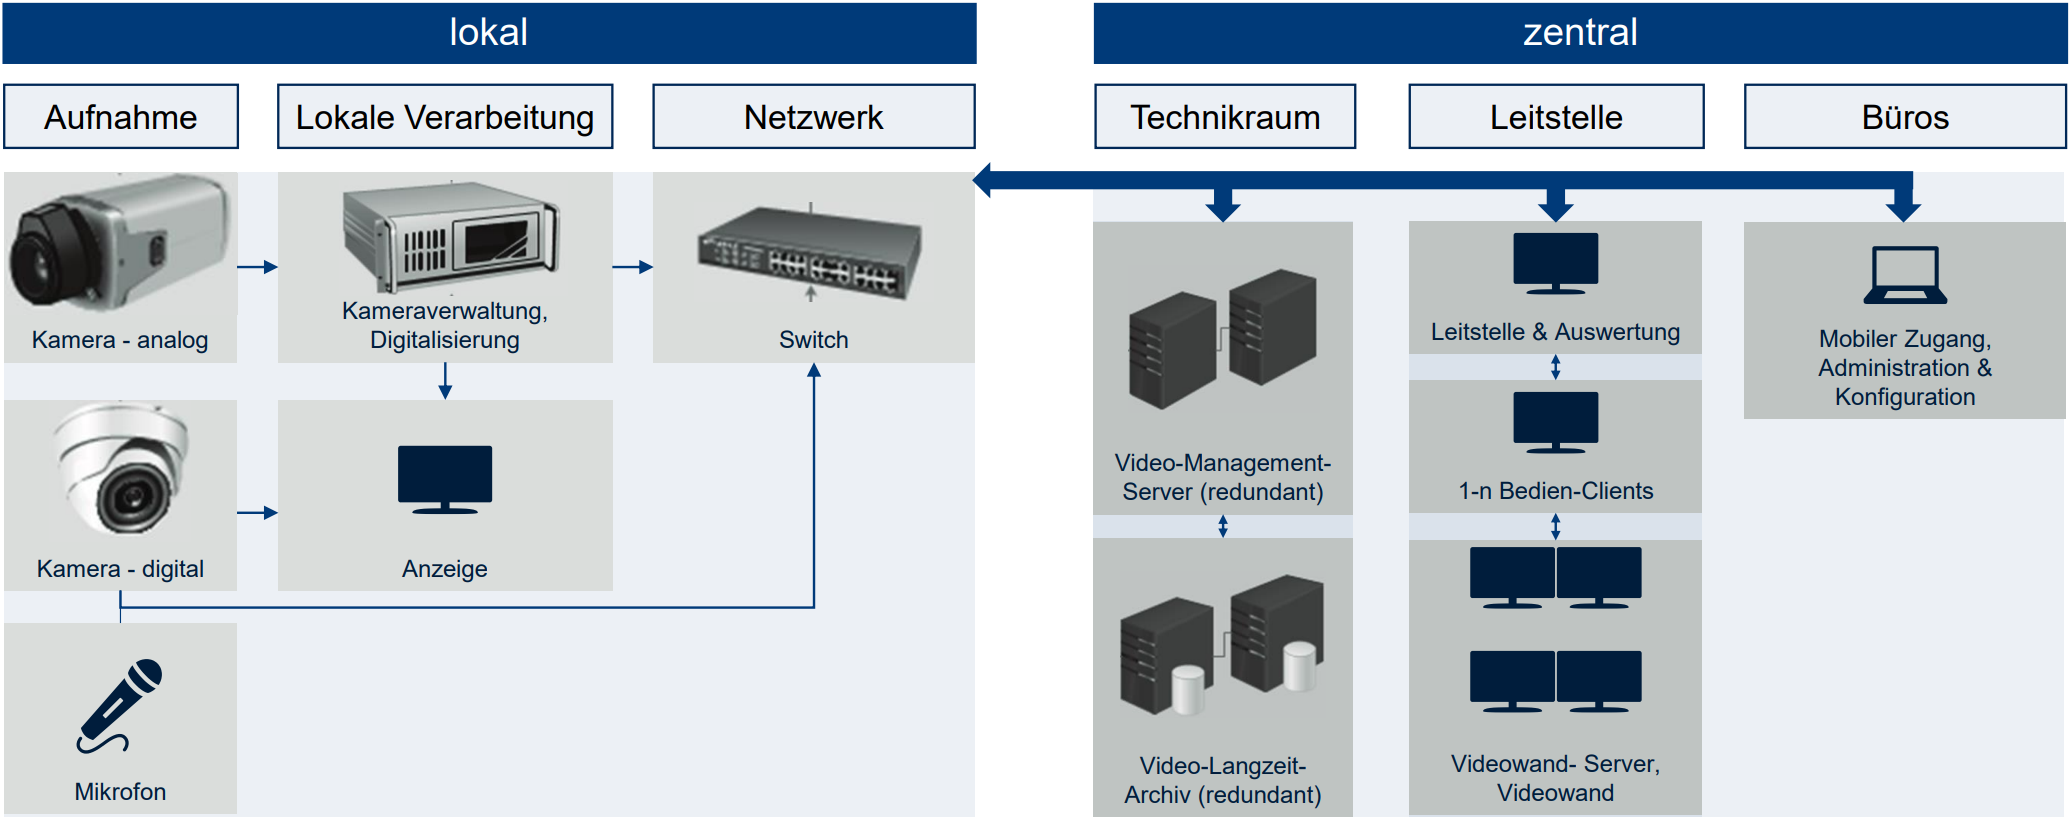
\includegraphics[width= 1\textwidth]{Bilder/architektur.png}
        \caption{Aufbau eines typischen Systems \cite{LandesbeauftragtefurdenDatenschutzBadenWurttemberg.2015}}
        \label{fig:architektur}
    \end{center}
\end{figure}
Die genaue Implementierung eines Systems kann abweichen, wichtig sind aber die Aspekte der Netzwerkübertragung und zentralen Auswertungsstelle für mehrere Kamerabilder.

\section{Security}

\subsection{Risikoidentifizierung}
\subsection{Konkretes Szenario}
\subsection{Maßnahmen}
\section{Privacy}

\subsection{Risikoidentifizierung}
\subsection{Konkretes Szenario}
\subsection{Maßnahmen}
\section{Fazit}
Die Fahrgastüberwachung im ÖPNV ist aus vielerlei Hinsicht ein prekäres Thema. Die einzige Kontrollmöglichkeit über das Vermeiden einer Aufzeichnung ist die Vermeidung der Verkehrsmittel, was für viele Menschen
nicht umsetzbar ist.

Weiterhin gibt es oft nur wenig Transparenz von Seiten der Verkehrsbetriebe zu der Menge der gesammelten Daten sowie der Art der Verarbeitung. Über den Link des in Abbildung \ref{fig:hinweis}
dargestellten Schildes wird nur auf die Homepage des Verkehrsbetriebes verwiesen, ohne konkrete Informationen zu liefern. Auch über die in Abschnitt \ref{abschnitt:technisch} beschriebene
Verwendung von Mikrofonen oder in Abschnitt \ref{abschnitt:massnahmen} vorgeschlagenen internen Prozesse zur Sicherstellung des Datenschutzes wird wenig aufgeklärt.

Dem gegenüber steht die große Angriffsfläche, auf welche auf verschiedene Arten und mit unterschiedlicher Motivationen zugegriffen werden kann.


\begin{thebibliography}{99}
    \bibitem{ref_article1}
    Author, F.: Article title. Journal \textbf{2}(5), 99--110 (2016)

    \bibitem{ref_lncs1}
    Author, F., Author, S.: Title of a proceedings paper. In: Editor,
    F., Editor, S. (eds.) CONFERENCE 2016, LNCS, vol. 9999, pp. 1--13.
    Springer, Heidelberg (2016). \doi{10.10007/1234567890}

    \bibitem{ref_book1}
    Author, F., Author, S., Author, T.: Book title. 2nd edn. Publisher,
    Location (1999)

    \bibitem{ref_proc1}
    Author, A.-B.: Contribution title. In: 9th International Proceedings
    on Proceedings, pp. 1--2. Publisher, Location (2010)

    \bibitem{ref_url1}
    LNCS Homepage, \url{http://www.springer.com/lncs}. Last accessed 4
    Oct 2017
\end{thebibliography}

\end{document}